% !TeX root = ../thuthesis-example.tex

\chapter{可预测预训练--可复用扩展定律与高效退火迭代}
% \thusetup{
%   cite-style = super,
% }

上一章介绍了使用超参数可扩展策略进行大语言模型预训练以节省模型的超参调优时间,以及使用性能扩展定律用来准确预测训练完成后的下游任务性能。本章中,我们将继续探索可预测预训练,侧重在高效测量扩展定律和进行扩展实验迭代本身。本章中,我提出了一种新的学习率调度策略,不仅能取得更好的效果,并且使得预测点的获取变得非常廉价,同时能提升不同预测点之间的规律性。基于这种策略,我们还可以进行高效的实验迭代,来获得性能更好的模型。最后我们使用这些策略训练了一个性能优异的24亿参数规模语言模型MiniCPM。


\section{可复用扩展定律}
扩展定律的建立需要进行大量实验。虽然实验的规模已经比训练最终模型小很多,但是仍然需要耗费大量的计算资源。为了减少实验的规模,本文提出了在数据维度可复用扩展定律。可复用扩展定律的核心思想是,通过一次实验,我们可以得到一个数据维度的扩展定律。在之前数据维度的扩展定律难以构建,原因主要是在一次训练过程中,损失并不遵循一个清晰的规律发展,而只有当训练完成,损失才会呈现标准的幂率扩展规律。针对这个问题,本文从主导训练过程中损失发展规律的学习率调度器开始展开研究。

\subsection{背景}
学习率调度器(Learning Rate Scheduler,简称LRS)通过调整训练不同阶段所使用的学习率,对模型性能至关重要。当前常用的学习率策略是余弦退火学习率调度器(Cosine LRS)~\citep{kaplan2020scaling, hoffmann2022training, rae2021scaling, touvron2023llama, bai2023qwen, almazrouei2023falcon},它在预热阶段后达到最大值,随后按照余弦曲线逐渐降低学习率。

余弦退火学习率调度器中的一个关键超参数是步长$T$,即余弦退火首次降至最小值的步数。通常,对于具有预定义训练步数的训练,$T$被设置为总训练步数$S$。一般认为,学习率应较高以实现充分探索。例如,~\citet{kaplan2020scaling}表明,当整个训练过程中的累计学习率增加时,损失会降低(见其论文中的图22)。这表明设置$T < S$并非最优。另一方面,~\citet{hoffmann2022training}有一个关键发现,即设置$T > S$会导致性能下降,而设置$S = T$则会提高训练效率,这证实了在整个训练过程中不应始终保持高学习率。为重现这些观察结果,我们在0.036B参数规模的模型上进行实验。我们按照下方的公式尝试$Cosine(T)$和$CosineLoop(T)$学习率调度器。结果见图\ref{fig:cosine_lr}。我们可以看到,当训练步数为$S = 20N, 40N, 60N, 80N$时,最低损失始终由$T = S$的$Cosine(T)$实现。$T < S$和$T > S$都不是最优的。

\begin{figure}[htbp]
    \centering
    % First minipage for the first figure
    \begin{minipage}{0.47\linewidth}
        \begin{equation*}
    \begin{aligned}
    & Cosine(T; s) = \\
    & \begin{cases}
       & \frac{s}{W} \eta, \quad s<W \\
       & 0.45\eta cos(\pi \frac{s}{T}) + 0.55\eta, \quad W < s < T \\
       & 0.1\eta,\quad  s > T \\
    \end{cases}
\end{aligned}
        \end{equation*}
    \end{minipage}
    \hfill % This adds a little space between the two figures
    % Second minipage for the second figure
    \begin{minipage}{0.52\linewidth}
             \begin{equation*}
    \begin{aligned}
    & CosineLoop(T; s) = \\
    & \begin{cases}
       & \frac{s}{W} \eta, \quad s<W \\
       & 0.45\eta cos(\pi \frac{s}{T}) + 0.55\eta, \quad W < s  \\
    \end{cases}
\end{aligned}
        \end{equation*}
    \end{minipage}
\end{figure}

\begin{figure}
    \centering
    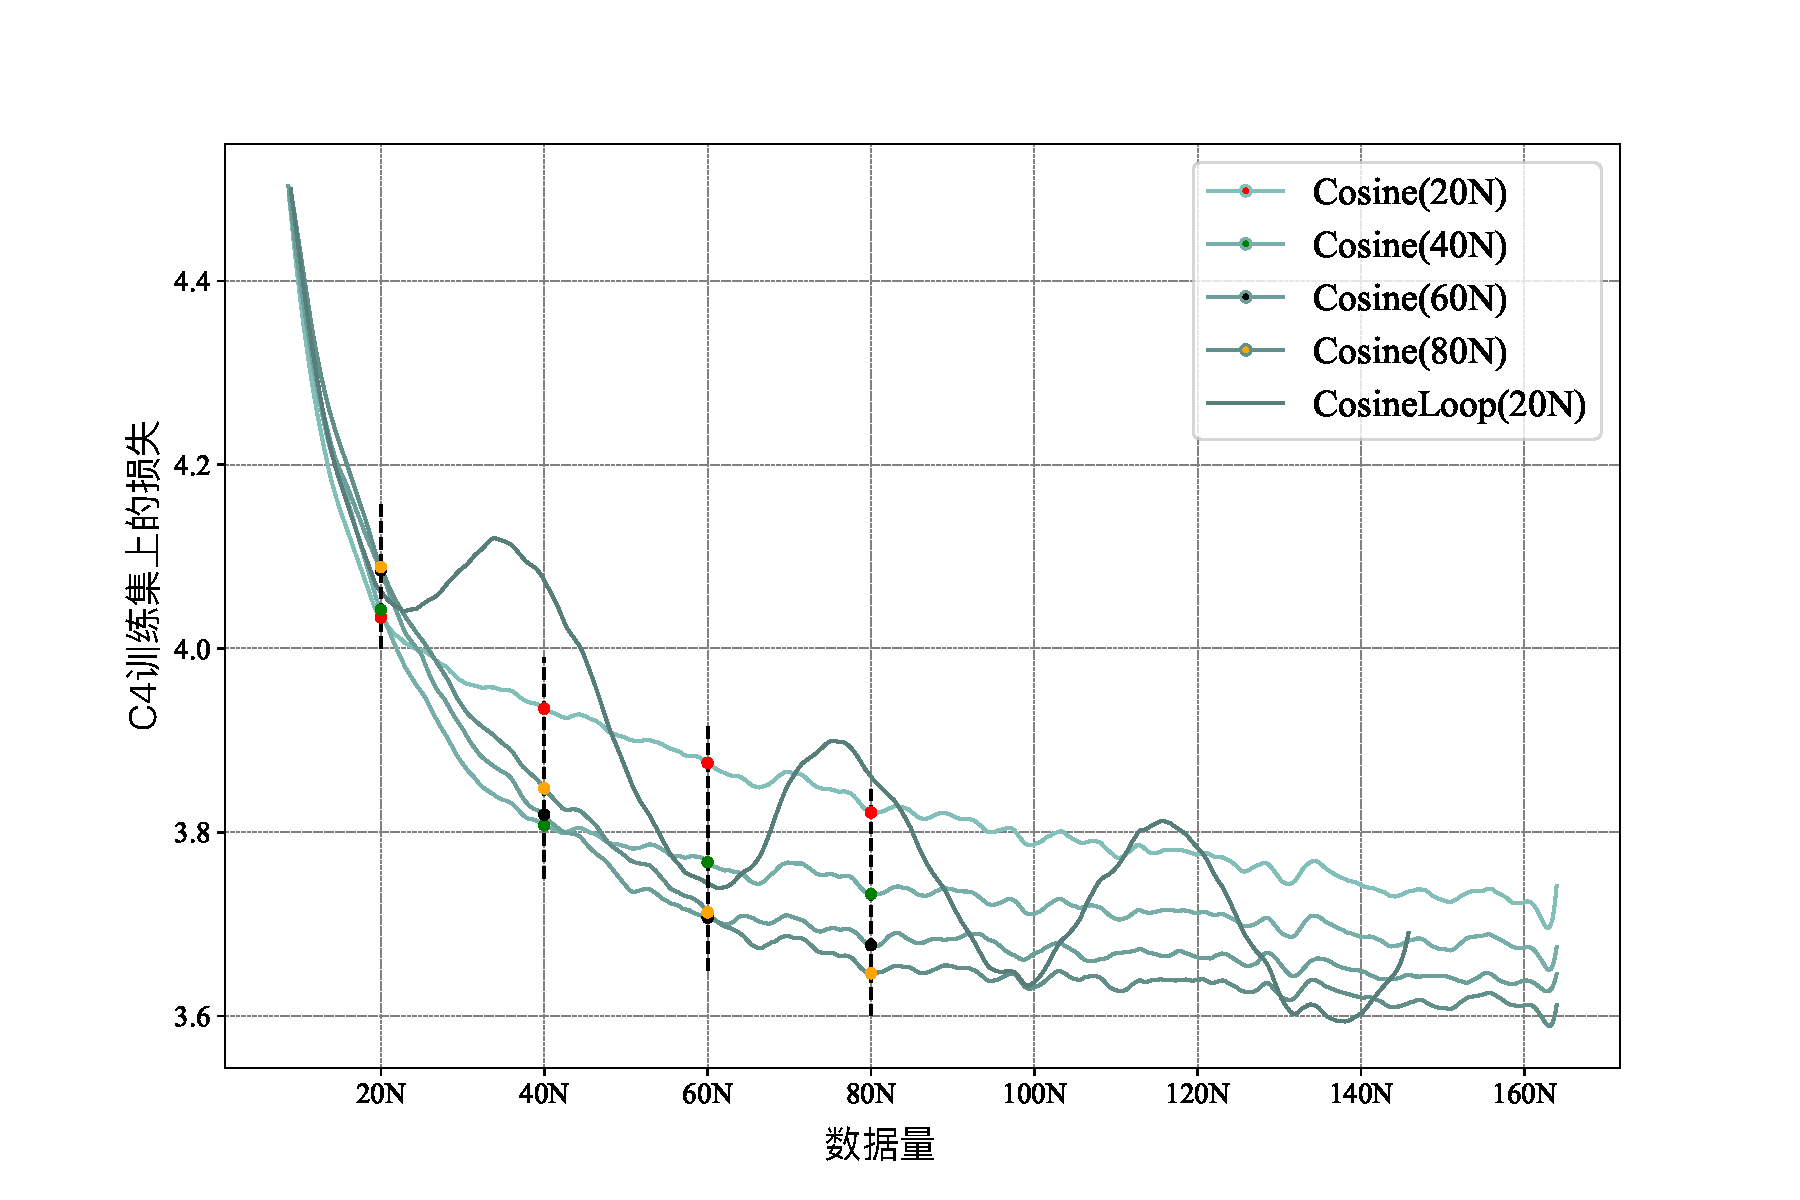
\includegraphics[width=0.9\linewidth]{minicpmFig/cosine_2024-03-26_15-36-16.zh.pdf}
    \caption{不同周期的余弦学习率调度器}
    \label{fig:cosine_lr}
    \vspace{0.47cm}
\end{figure}

我们假设当$T = S$时余弦退火学习率表现出色是基于以下两个原因:(1) 与$T < S$以及其他如线性学习率调度器(Linear LRS)相比,$T = S$的余弦退火学习率调度器具有更长的“高学习率”训练持续时间。这种高学习率可能有助于模型找到更好的全局最优解。(2) 与$T > S$的余弦退火学习率调度器以及固定学习率调度器相比,$T = S$的余弦退火学习率调度器具有更彻底的学习率衰减阶段。这种学习率衰减可能涉及独特的训练动态,使模型能够找到更好的局部最优解。

\subsection{方法}
\subsubsection{WSD学习率调度器}
鉴于上述观点,我们提议明确地将训练阶段划分为高学习率阶段和学习率衰减阶段。我们将其命名为预热-稳定-衰减(Warmup-Stable-Decay,简称WSD)学习率调度器。特别地,WSD学习率调度器包含三个阶段:预热阶段(结束步数记为$W$)、稳定训练阶段(结束步数记为$T$)以及剩余的衰减阶段。WSD的函数形式为:

\begin{equation}
    \text{WSD}(T; s) = \begin{cases}
       & \frac{s}{W} \eta, \quad s<W\\
       & \eta, \quad W < s < T \\
       & f(s-T)\eta,\quad T < s < S\\
    \end{cases}
\end{equation}
其中$0 < f(s - T) \leq 1$是关于$s$的递减函数,$\eta$是最大学习率。通常,只要预热阶段足够,其对性能影响不大,因此,在后续讨论中我们省略$W$。为简化表述,我们将使用明确的停止点来表示WSD。 图\ref{fig:learning_rate_scheduler_diagram} 将WSD学习率调度器的图像和Cosine调度的图像进行了比较。不同结束步数的WSD学习率调度共享同样的稳定训练阶段。

\begin{figure}[!htbp]
    \centering
    % First minipage for the first figure
        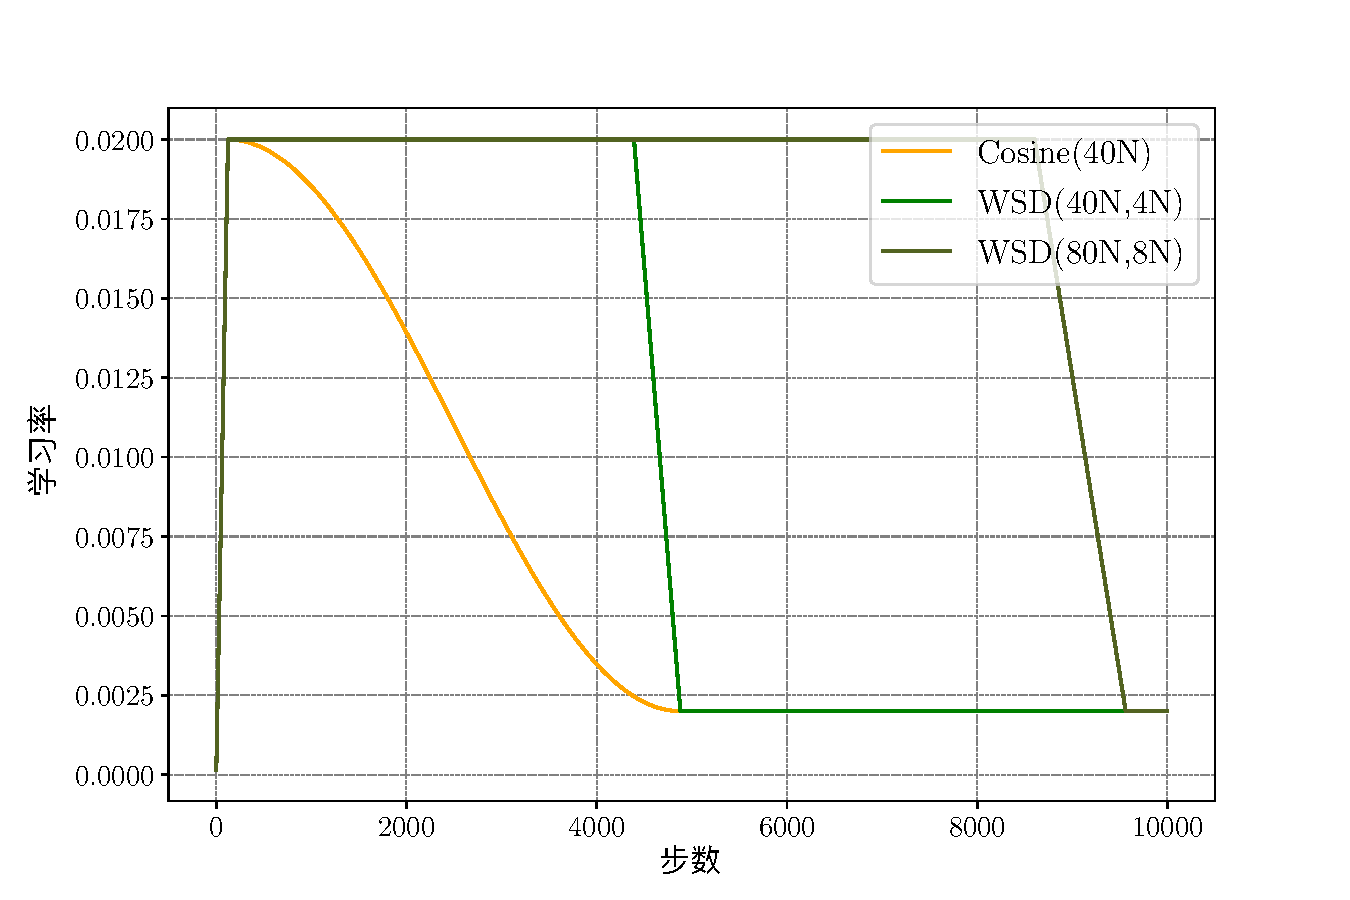
\includegraphics[width=0.8\linewidth]{minicpmFig/lr.zh.pdf}
        \caption{WSD调度器图像与余弦调度器图像比较}\label{fig:learning_rate_scheduler_diagram}
\end{figure}

\begin{figure}[htbp]
    \centering
    % First minipage for the first figure
    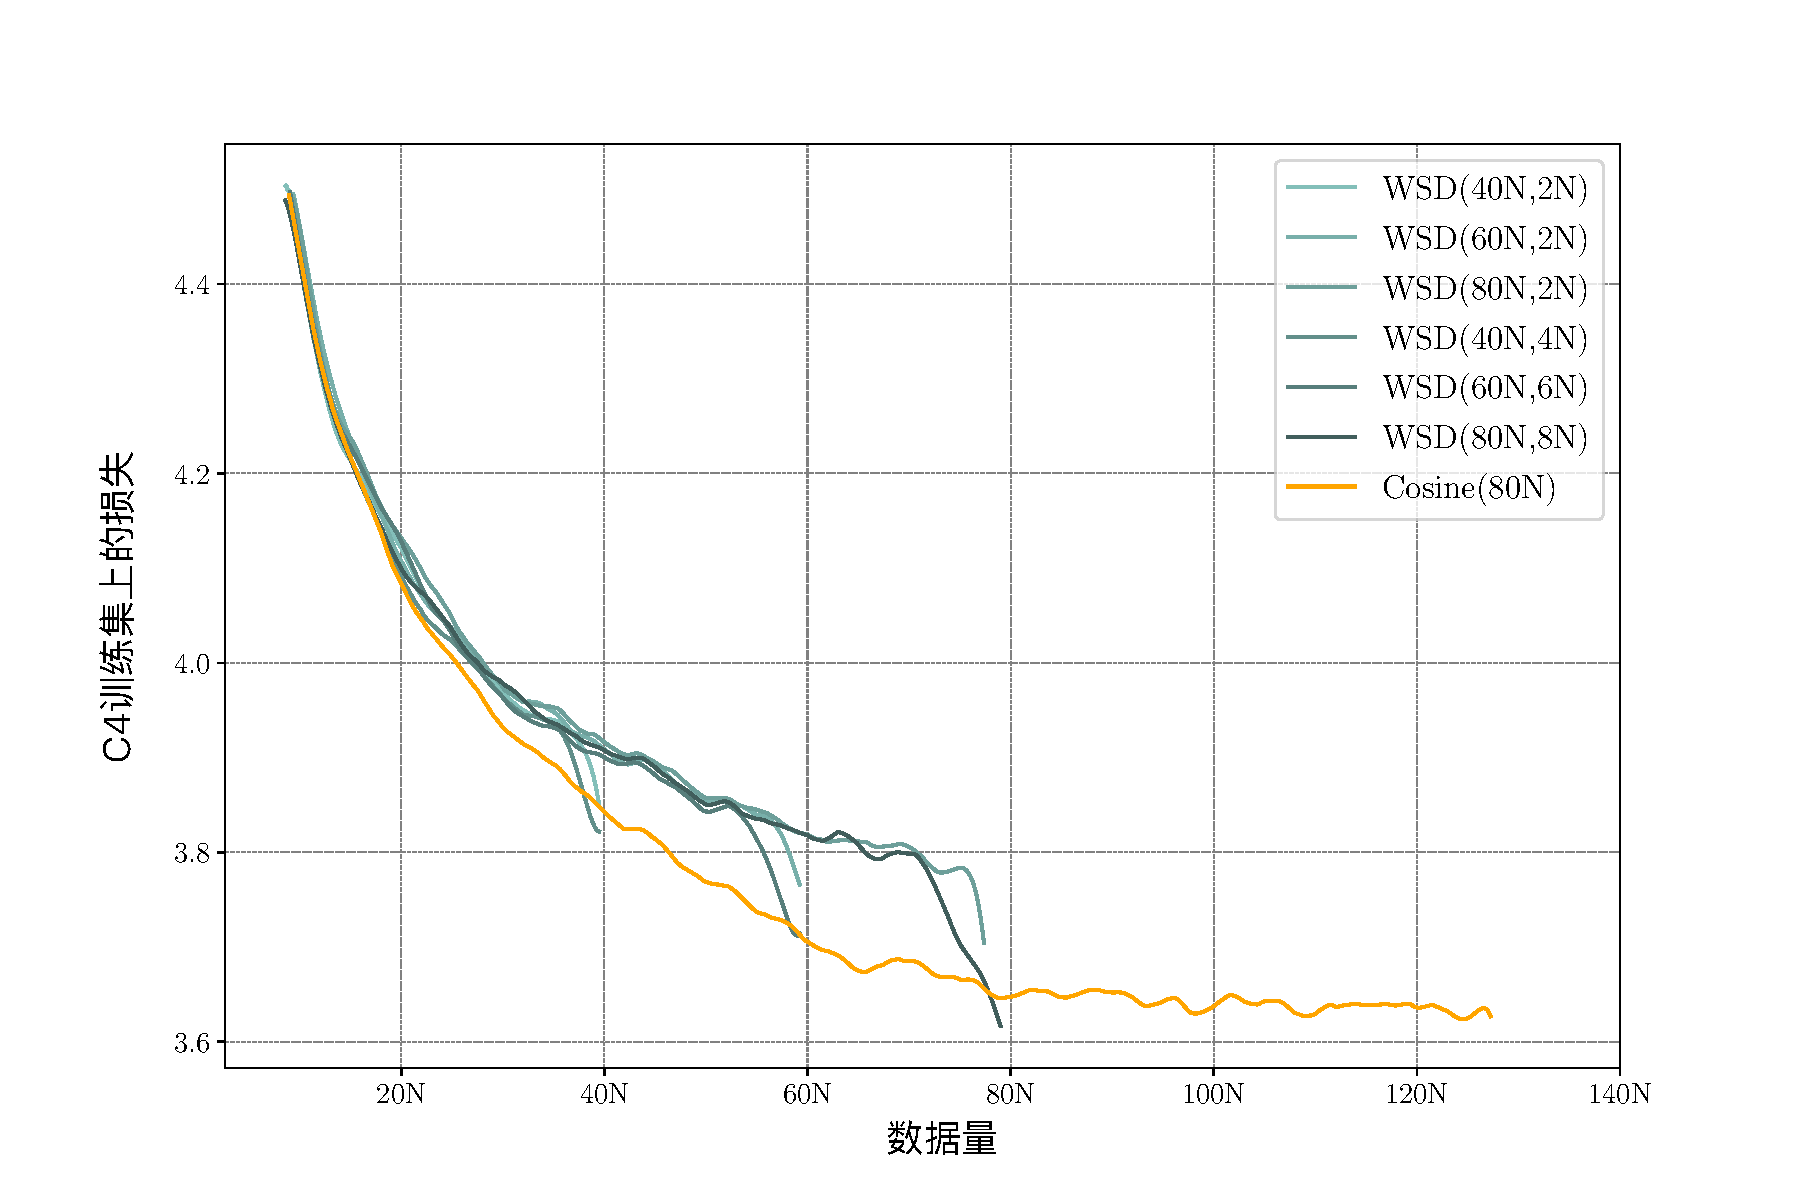
\includegraphics[width=0.75\linewidth]{minicpmFig/WSD_diff_dcay.zh.pdf}
    \caption{WSD学习率调度的衰减阶段的模型训练损失突然下降}
    \label{fig:wsd_diff_dcay}
\end{figure}

\begin{figure}[htbp]
    \centering
    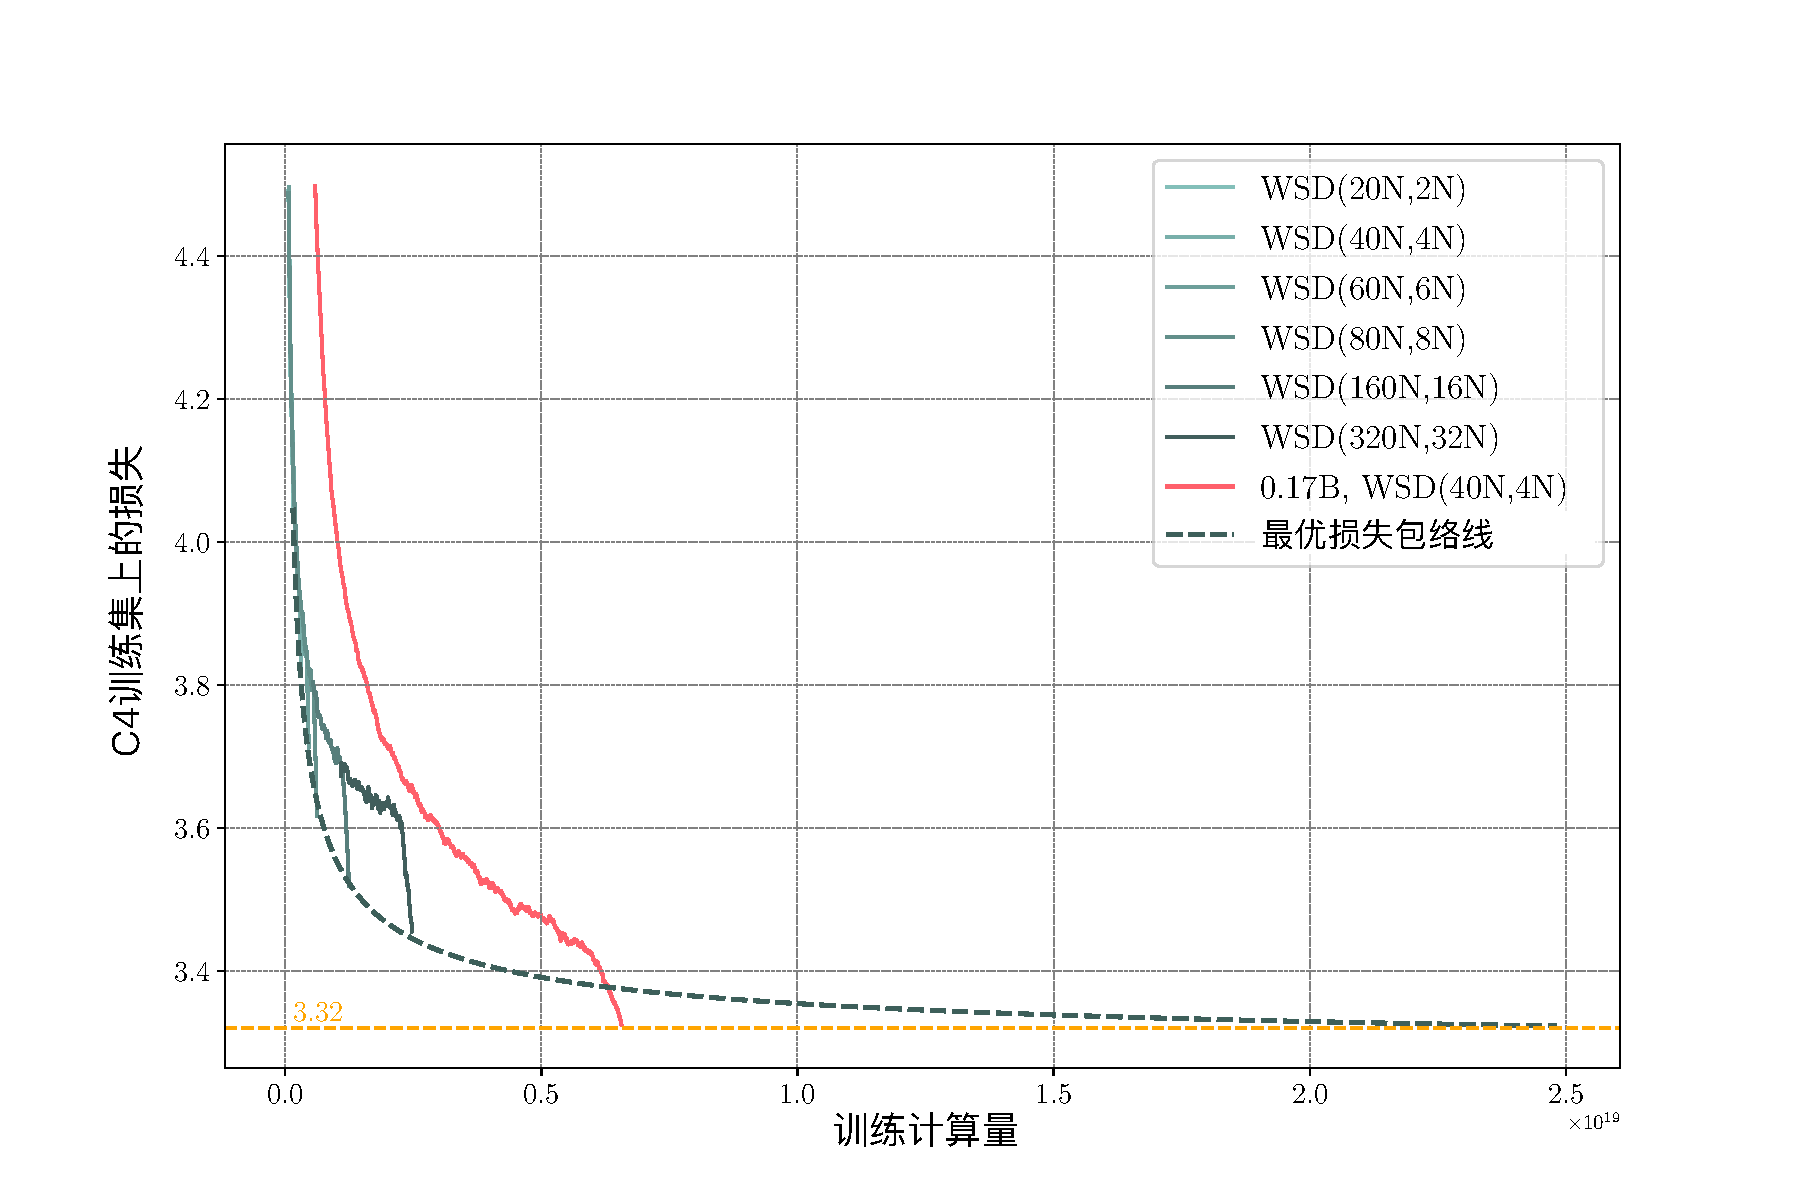
\includegraphics[width=0.8\linewidth]{minicpmFig/continuous_train.zh.pdf}
    \caption{使用WSD调度对固定规模模型进行持续训练}
    \label{fig:continuoustrain}
\end{figure}


\subsection{实验}
\label{sec:wsd_experiments_continoustrain}
接下来,本文展示WSD学习率调度器的几个实验结果。

\textbf{衰减阶段损失急剧下降。} 本文在0.036B参数规模的模型上尝试WSD学习率调度器。如图\ref{fig:wsd_diff_dcay}所示,在衰减阶段,随着学习率开始下降,损失经历显著快速下降,并迅速降至与$T = S$时的余弦学习率调度器相等或更低的水平。同时,本文可以重用衰减前的模型,并以之前的高学习率继续训练。经过更多步训练$S'$后,进行退火操作,以达到与$Cosine(S')$时的Cosine LRS相同的损失。这验证了本文的假设,即训练阶段可以明确地划分为稳定训练阶段和衰减阶段。

\textbf{10\%的步数就足够。} 从两阶段训练的角度来看,缩短衰减阶段将极大有利于对稳定训练的不同模型检查点进行快速测试。因此,本文进行实验,从相同的稳定训练检查点开始,但具有不同的衰减步数。同样如图\ref{fig:wsd_diff_dcay}所示,在40N、60N和80N训练数据的所有三个稳定训练检查点中,使用总词元数10\%的衰减量就足以获得最佳结果,而使用总词元数2.5\%的衰减量则无法达到。因此,在后续的训练实验中,本文使用约10\%的衰减量以确保充分收敛。

\textbf{WSD学习率跳读下的有效数据扩展。} 使用WSD学习率调度,本文可以持续训练语言模型直至极度收敛。为进一步展示将固定规模模型训练至收敛的潜力,本文比较了使用40N数据对0.036B的LM和0.17B模型进行持续训练的情况。
在图\ref{fig:continuoustrain}中,绿线表示使用不同稳定训练词元数训练的0.036B模型。尽管0.036B系列的最后一个点所使用的训练词元数比Chinchilla最优值20N~\citep{hoffmann2022training}多得多,但它仍有性能提升空间。

\definecolor{darkgreen}{rgb}{0.0, 0.5, 0.0}

为找到对这个固定规模的语言模型进行持续训练的极限,本文估计在持续训练过程中模型的最优性能如何随其计算量变化。这里的最优性能,是指通过$\text{WSD}(D, 0.1D)$得到的训练词元$D$的损失。对于一系列的$D$,这些损失将形成最优损失包络线。由于不确定损失包络线的函数形式,我们尝试了两个拟合公式:(1) 指数形式:$L(C) = \alpha e^{-\beta C} + L_0$ 以及 (2) 幂律形式:$L(C) = \beta C^{-\alpha} + L_0$。这两个函数的拟合结果展示在图\ref{fig:fit_continue_train}中。拟合曲线以\textcolor{darkgreen}{绿色}虚线显示。图中的每个点是WSD学习率调度器中衰减阶段的结束点,对应不同的结束步数。拟合结果表明,幂率扩展定律对于持续训练仍是最佳的。 



\begin{figure}[!htbp]
    \centering
    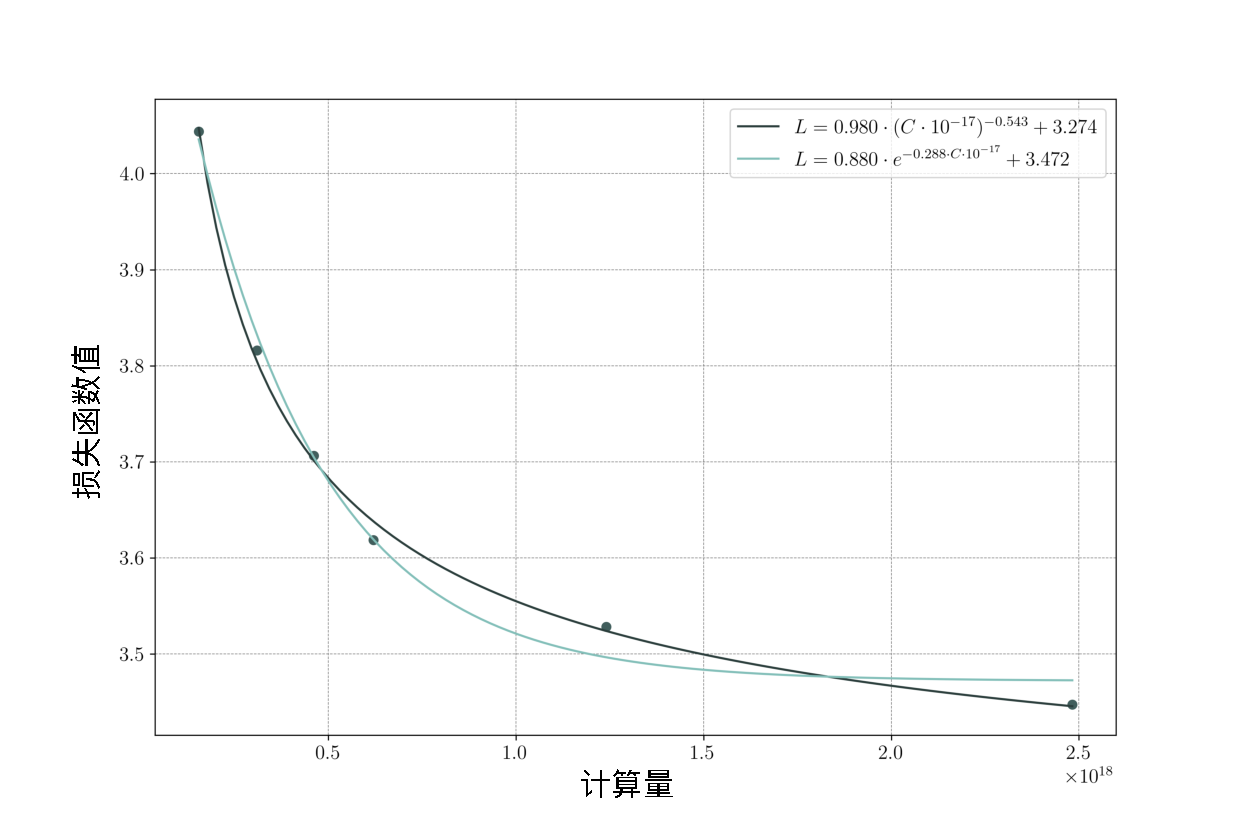
\includegraphics[width=0.85\linewidth]{minicpmFig/fit_continuetrain.zh.pdf}
    \caption{数据扩展维度的不同拟合函数的拟合效果}
    \label{fig:fit_continue_train}
\end{figure}



为直观估计和理解对这样一个固定规模模型进行持续训练的效果,本文还使用$WSD(40N, 4N)$训练了一个0.17B模型,在图\ref{fig:continuoustrain}中以\textcolor{pink}{粉色}显示。我们可以看到,一个0.036B模型在训练计算量有可接受的增加(约4倍)的情况下,能够达到与0.17B模型相当的性能,同时节省大量推理计算量~\citep{sardana2023beyond}(每次推理调用节省约5倍),这表明其是一种更好的推理-计算最优设置~\citep{sardana2023beyond}。 


\subsubsection{使用WSD学习率调度器衡量扩展定律}
\label{scalinglawwsdlrs}
接下来,我们回到扩展定律的测量上。在本节中,我们目标是测量得到一个计算最优的数据模型比例 尽管由于不同模型系列的配置各异,这些扩展定律在具体系数上存在差异,但计算最优数据与模型的比率在不同的扩展定律函数中仍是一个有意义的指标,它 “忽略” 了损失的具体数值。关于这一比率,\citet{kaplan2020scaling}认为模型规模增加十倍应等同于数据规模增加一倍。相反,\citet{hoffmann2022training}主张模型大小与数据大小的扩展率相同。此外,当前的模型如LLama-2\cite{touvron2023llama},所使用的训练数据比 \citet{hoffmann2022training} 所宣称的要多得多,却仍能带来显著的性能提升,这表明其数据与模型的比率更高。

这种尚未解决的不确定性源于传统扩展实验中训练多个不同大小模型和数据规模所固有的挑战。此前,如果在一种数据规模上训练一种模型规模的平均成本为 $C$,那么使用 $m$ 种模型规模和 $m$ 种数据规模进行扩展实验大约需要 $O(m^2)C$ 的成本。也就是说,比率需要同时进行两个维度的扩展测量,需要消耗平方量级的复杂度,是比较消耗资源的。

本文使用WSD调度器作为一种有效的方法,以线性成本($O(mC)$)来探索该比率。由于WSD调度器具有从任意步数的稳定阶段检查点衰减后达到余弦退火学习率调度器最优损失的优势,我们现在能够精确测量最优扩展属性,而无需将模型从头开始训练到不同数量的词元,从而使沿数据轴的扩展定律测量效率大大提高。

我们通过训练6种规模从0.04B到2B的小语言模型(SLMs)来沿数据轴和模型轴测量扩展定律,每种模型在稳定训练阶段都有6个从 $10N$ 到 $60N$ 数据的检查点开始衰减的模型($N$ 为相应的模型规模)。最终损失在五个留出的评估数据集上进行评估。为了在模型使用不同分词器时能够比较损失,我们按照~\cite{achiam2023gpt},以字节数而非词元数来取损失的平均值。每对数据规模和模型规模的最终损失如图\ref{fig:individual_task_datascalinglaw}中的蓝线所示。除了0.11B和0.25B模型的最后检查点外,拟合结果令人满意。 

然后,我们按照 ~\cite{hoffmann2022training} 使用scipy的\texttt{curvefit}函数,用模型规模 $N$ 和数据规模 $D$ 对损失进行拟合:

\begin{equation}
    L(N, D) = C_NN^{-\alpha} + C_DD^{-\beta} + L_0
\label{equ:scalinglaw}
\end{equation}

每个数据集和每个检查点沿数据轴的拟合曲线如图\ref{fig:individual_task_datascalinglaw}中的橙线所示。沿数据和模型双维度扩展的汇总图如\ref{fig:wsd_optimalscalinglaw}。x轴为计算量Flops,$C = 6ND$,每条线的颜色代表相同模型但具有不同的计算量Flops。我们可以看到,当Flops较小时,较小的模型表现优于较大的模型;而当Flops较大时,较小的模型表现较差。因此,不同规模的模型在图中计算最优区域附近会相互交叉。


\begin{figure}
    \centering
    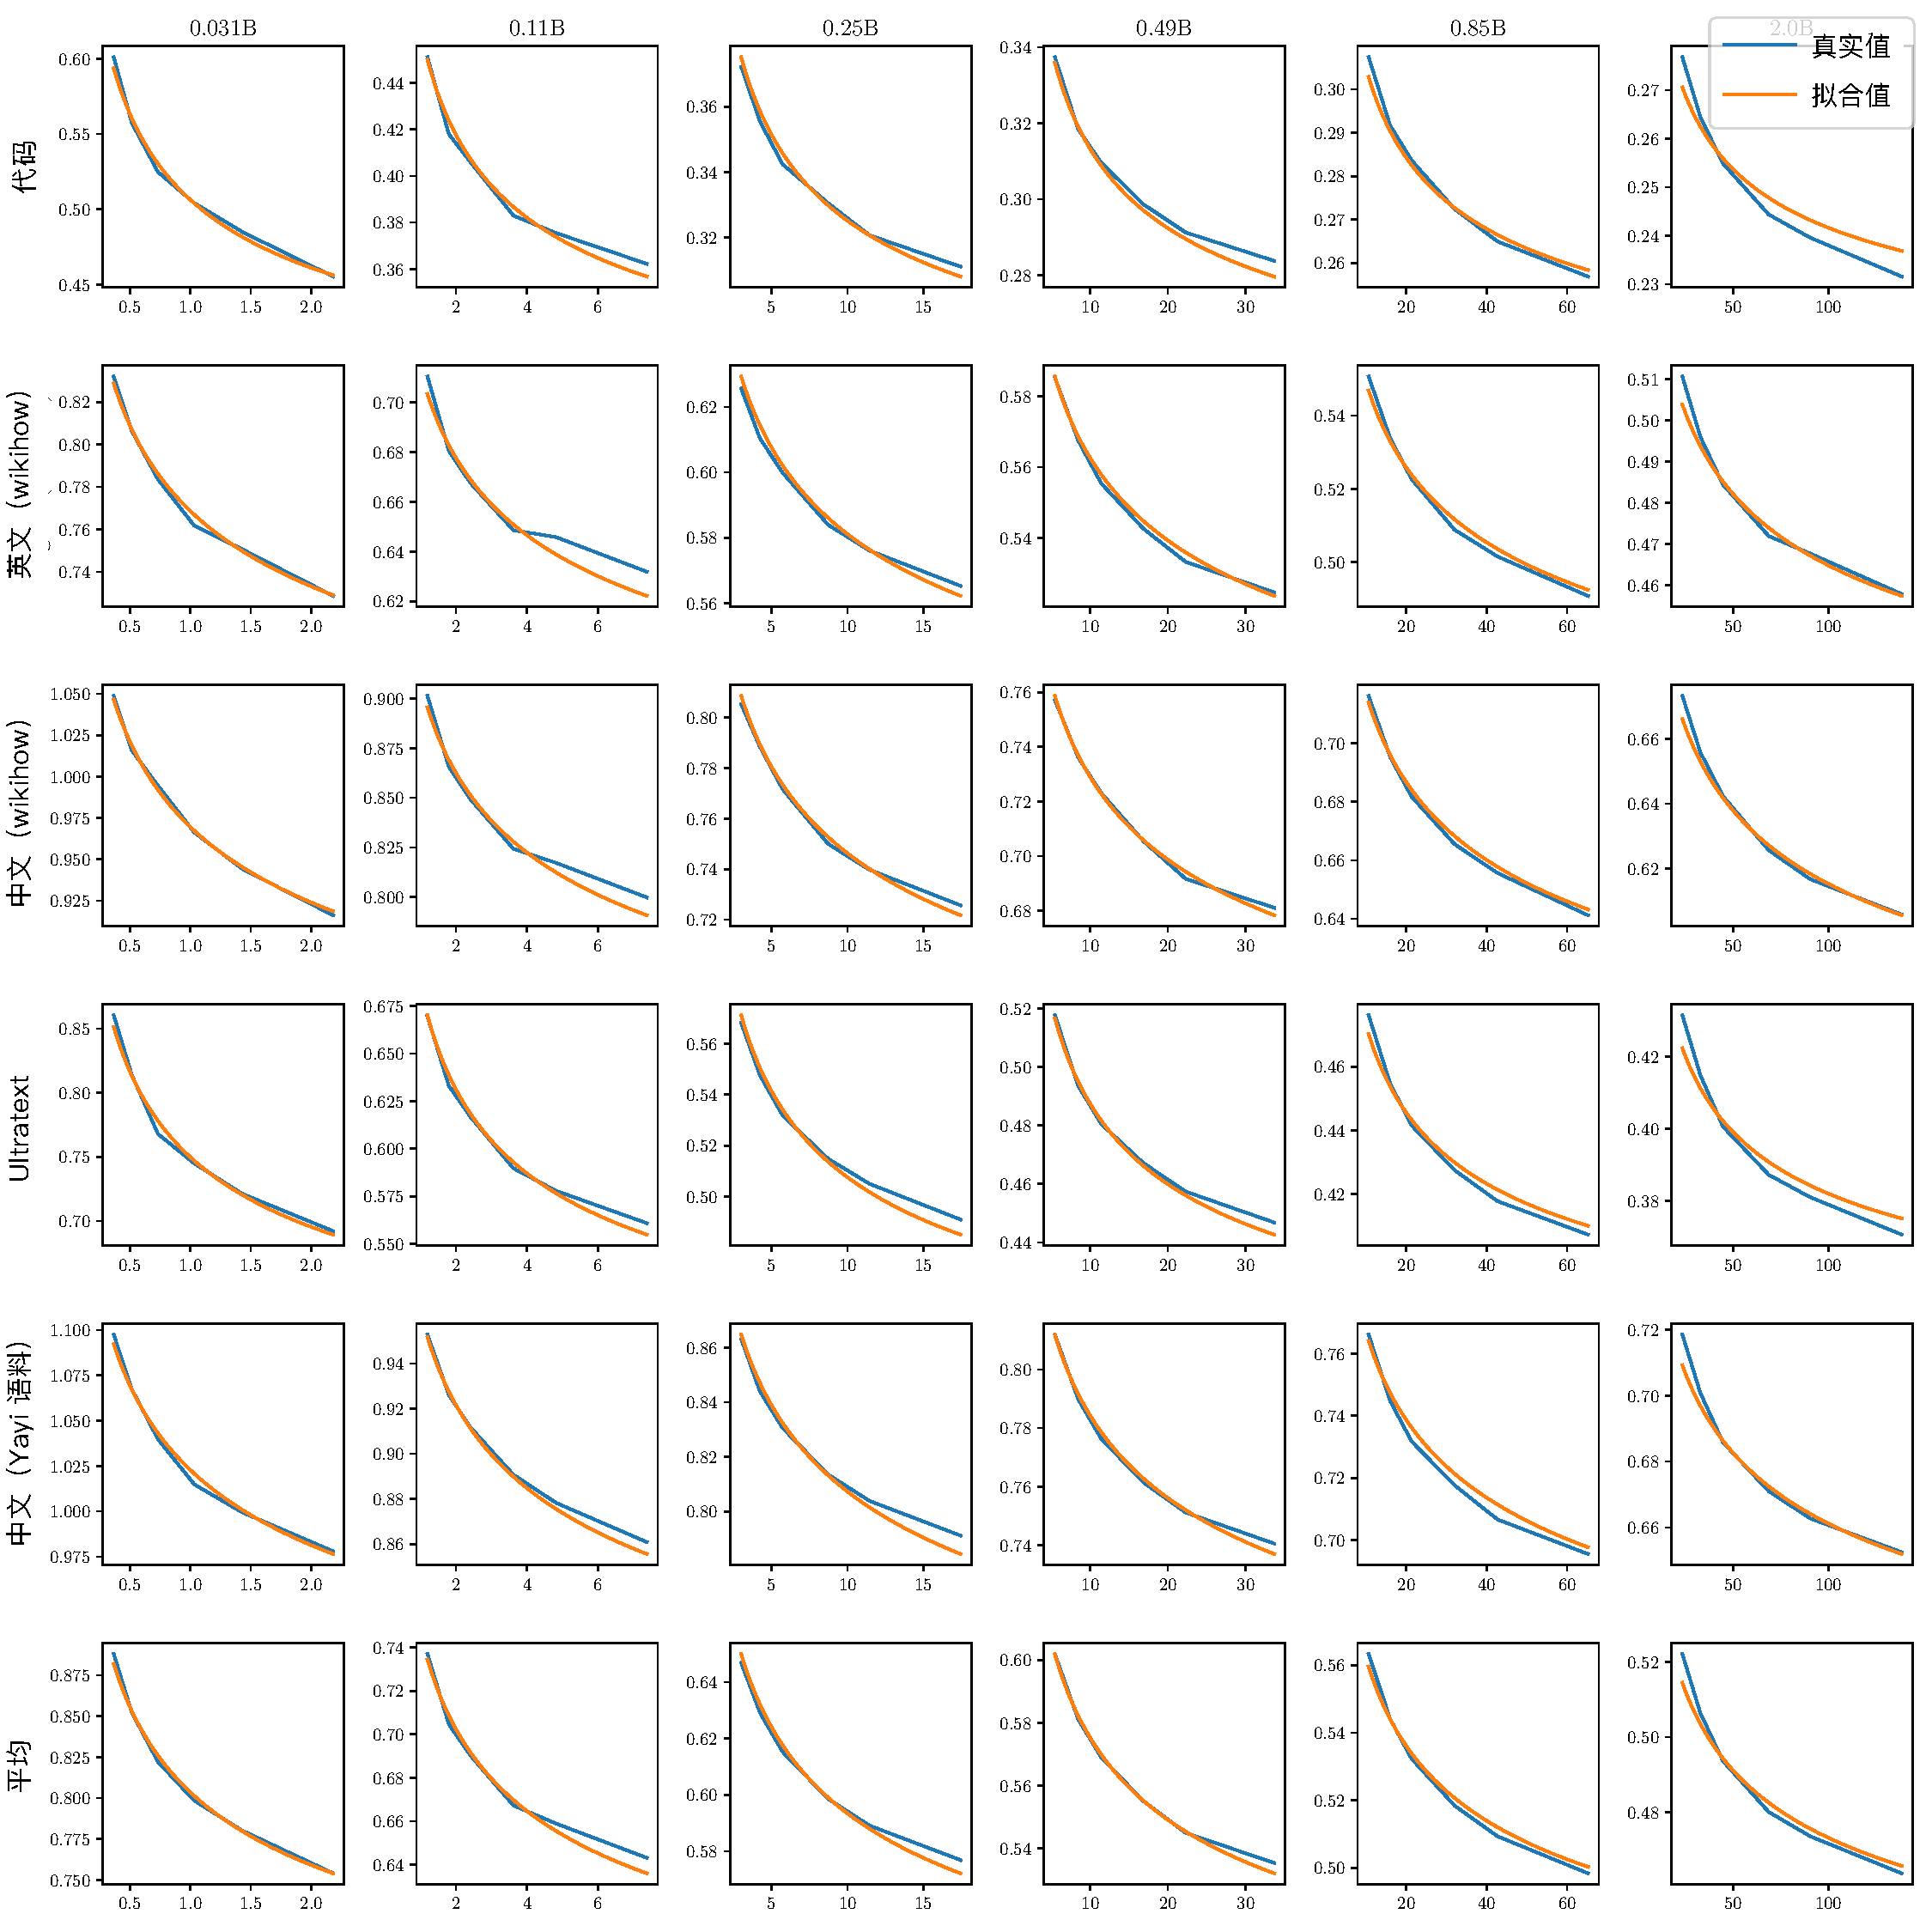
\includegraphics[width=1.0\textwidth]{minicpmFig/individual_task_datascalinglaw.zh.pdf}
    \caption{对每个模型和每个任务沿数据量轴绘制的拟合扩展定律}
    \label{fig:individual_task_datascalinglaw}
\end{figure}


\begin{figure}[!t]
    \centering
    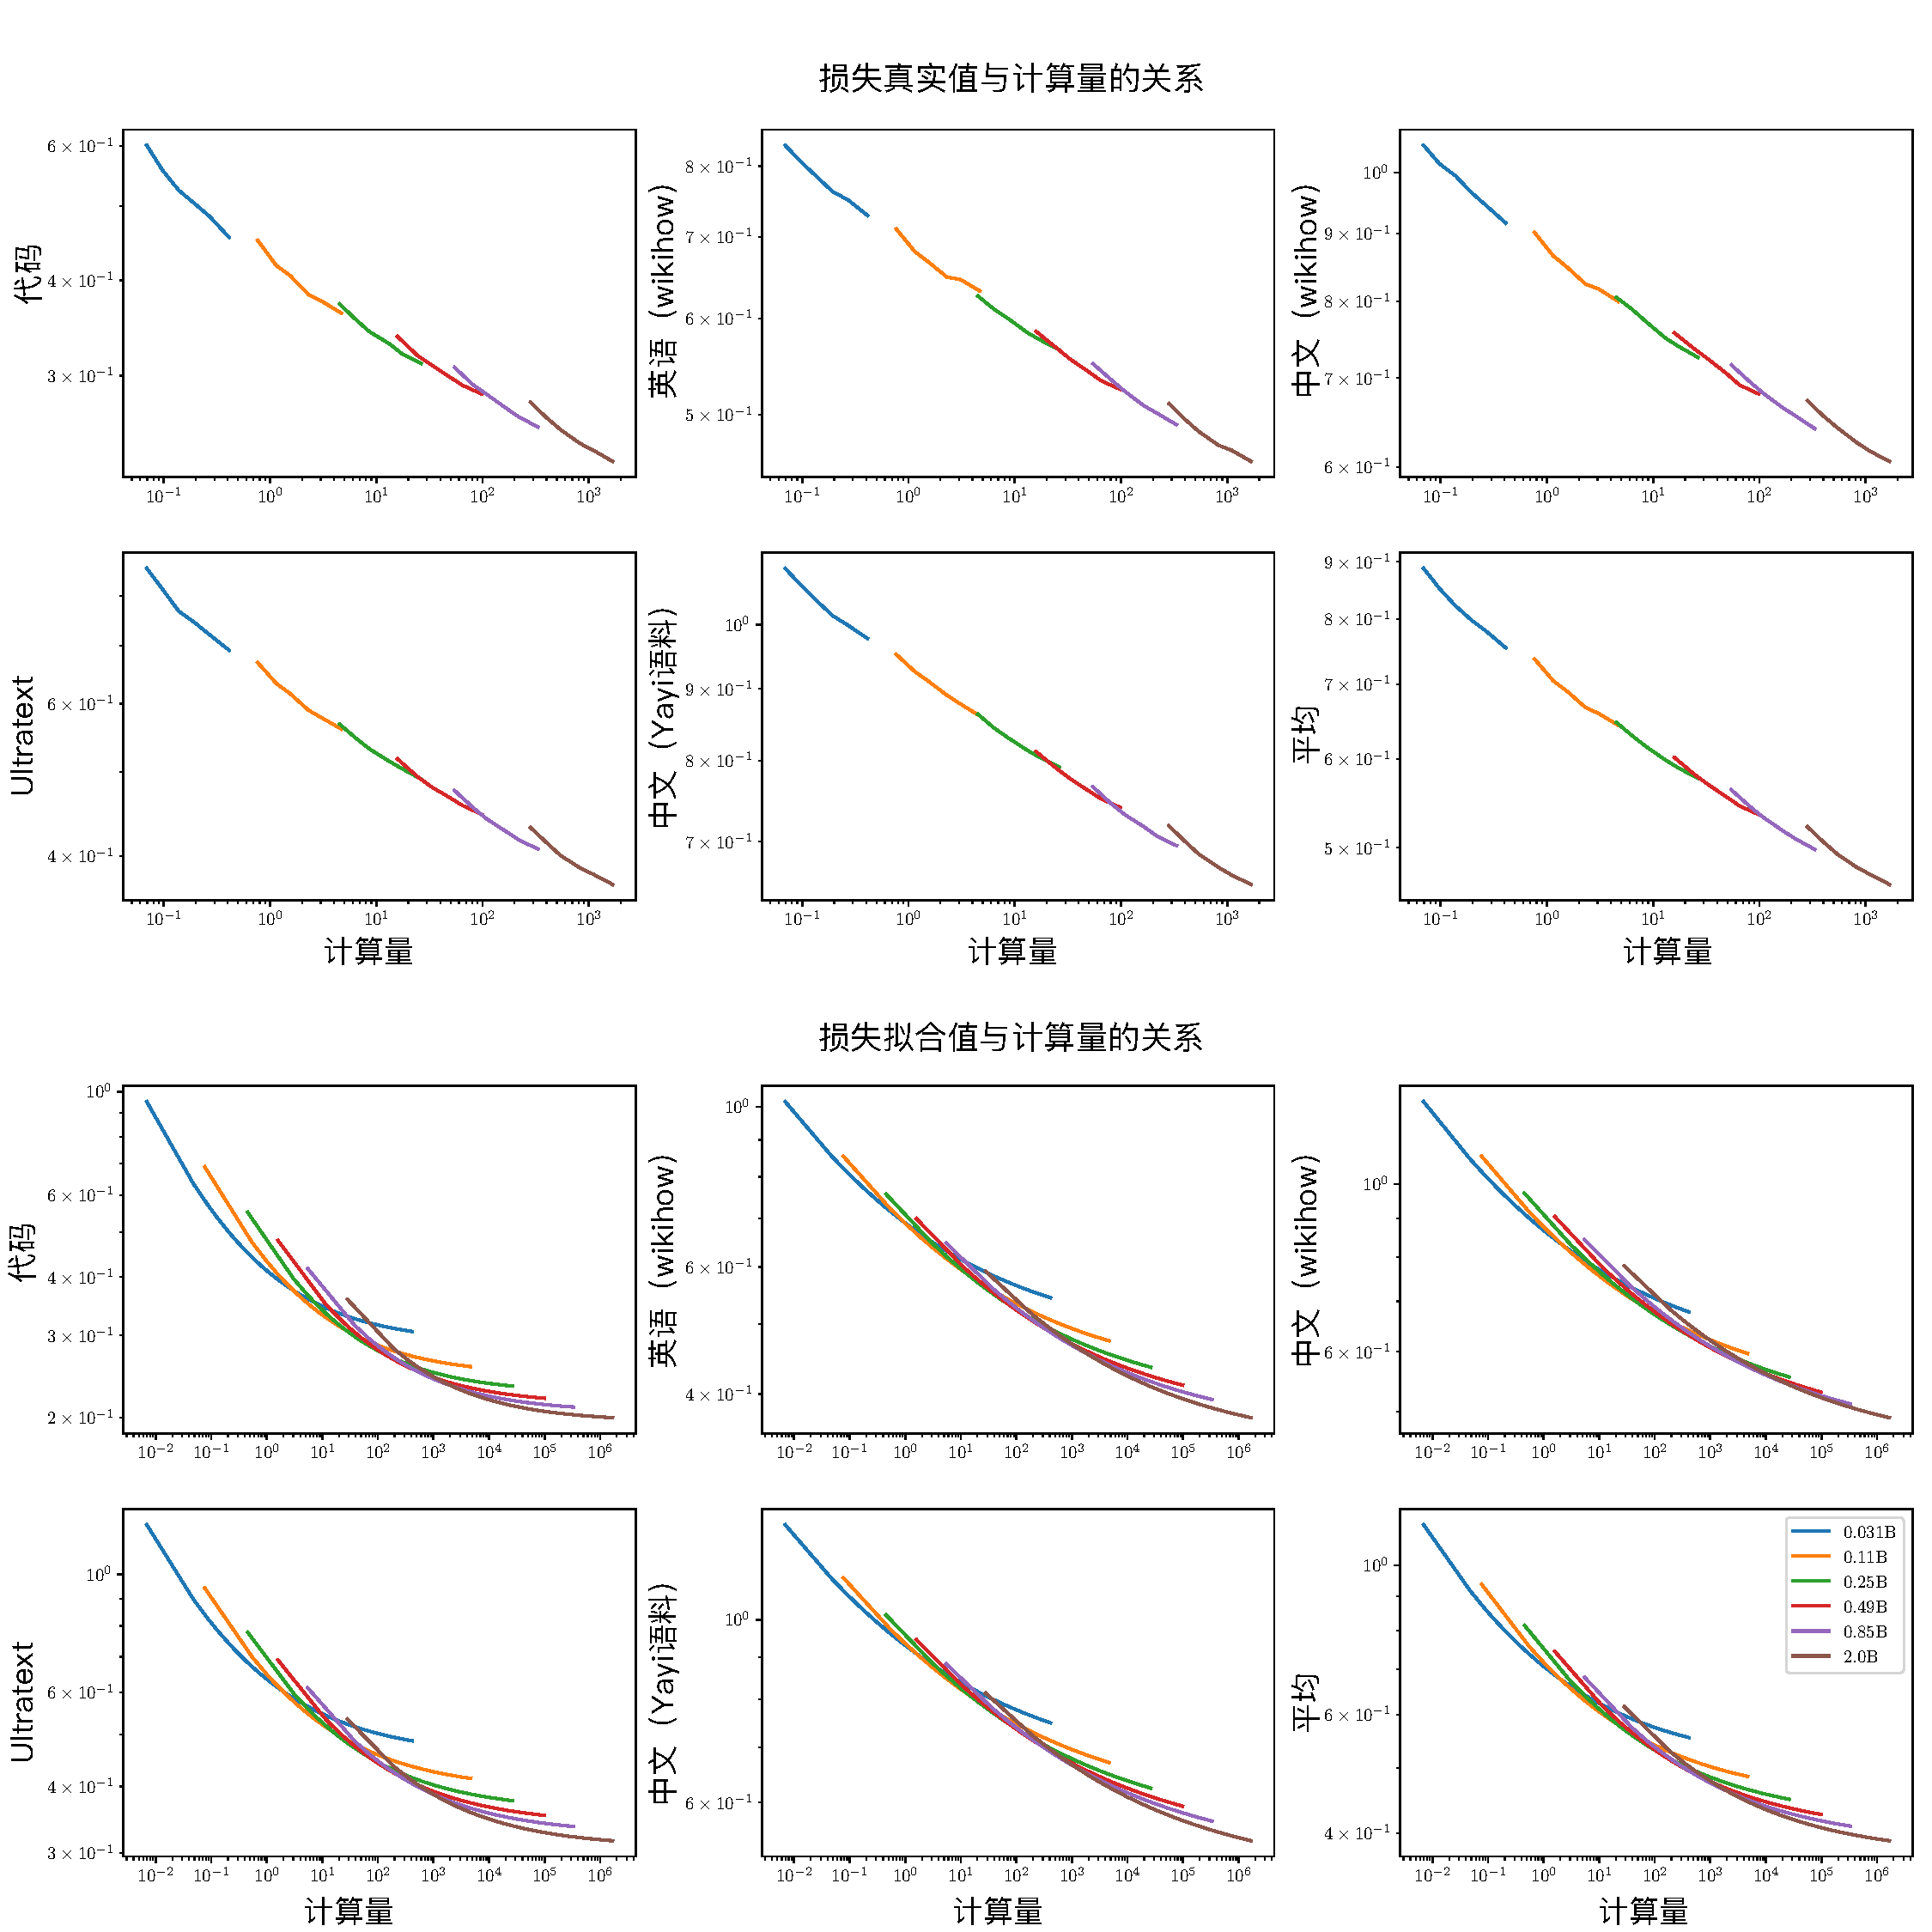
\includegraphics[width=\textwidth]{minicpmFig/lossvscompute_fitted_and_real.zh.pdf}
    \caption{使用WSD调度器的双维度扩展曲线图}
    \label{fig:wsd_optimalscalinglaw}
\end{figure}

在给定固定计算量 $C = 6ND$~\citep{rae2021scaling} 的情况下,我们得到最优模型规模 $N_{opt}$ 和数据集规模 $D_{opt}$ 为: 

\begin{equation}
    \frac{N_{opt}}{D_{opt}} = K^2\left(\frac{C}{6}\right)^{\eta},
\label{equ:computeoptimal}
\end{equation}


其中 $K = (\frac{\alpha C_N}{\beta C_D})^{\frac{1}{\alpha + \beta}} $,且 $\eta=\frac{\beta - \alpha}{\alpha + \beta}$。$N_{opt}$ 的推导紧密遵循 ~\cite{hoffmann2022training},将公式\ref{equ:scalinglaw} 中的 $D$ 替换为 $\frac{C}{6N}$,并在给定 $C$ 的情况下最小化 $L(N)$。$D_{opt}$ 的推导采用类似方法。 
从公式\ref{equ:computeoptimal} 可知,当 $\alpha = \beta$ 时,$N_{opt}/D_{opt}$ 为常数,支持了 ~\citet{hoffmann2022training} 的观点;当 $\alpha < \beta$ 时,我们应更强调参数扩展~\citep{kaplan2020scaling},反之亦然。 

本文进一步将损失与 $N$、$D$ 之间的拟合关系如图\ref{fig:wsd_optimalscalinglaw_contour} 中损失等值线图所示。水平线上的黑点表示相同模型规模下不同计算量中的衰减检查点。图例中的$C$为语义完整以Flops为单位表示,未使用EFlops单位。y轴上的$C$以EFlops为单位。每个子图中第一个文本框显示拟合扩展定律的方程。我们可以看到,在所有评估语料库中,$\beta < \alpha$。更具体地说,平均而言,$\alpha = 0.29$,$\beta = 0.23$,$K^2 = 0.01$,$\eta = -0.10$(注意 $N$ 在 $10^9$ 以下,$D$ 在 $10^9$ 以下,$C$ 在 $10^{18}$ 以下)。由于 $\alpha$ 略大于 $\beta$,这一结果表明,随着计算规模的变化,我们应比模型扩展更略微强调数据扩展,这与\citet{hoffmann2022training} 的观点一致。

至于具体的数据与模型的比率 $\frac{D_{opt}}{N_{opt}}$,我们注意到,尽管我们的结果与 \citet{hoffmann2022training} 中 $\frac{D_{opt}}{N_{opt}}$ 随计算量 $C$ 变化的趋势一致,但在计算最优区域仍存在巨大差距。具体而言,平均数据规模应比模型规模大192倍,而\citet{hoffmann2022training}中为20倍。我们注意到这与\ref{sec:wsd_experiments_continoustrain} 节和图\ref{fig:continuoustrain} 中的观察结果一致。




\begin{figure}[!t]
    \centering
    \includegraphics[width=1.0\textwidth]{minicpmFig/wsd_optimal_scaling_law.zh.pdf}
    \caption{使用WSD调度器进行扩展实验的拟合结果的等高线图}
    \label{fig:wsd_optimalscalinglaw_contour}
\end{figure}



\subsubsection{Llama2数据与模型比率的分析}
关于与Chinchilla最优的 $\frac{N_{opt}}{D_{opt}}$ 存在较大偏差,我们注意到他们的扩展实验是在一个不是非常新的配置下进行的。为了与更新的配置(如Llama2~\citep{touvron2023llama})进行比较,我们从Llama2论文中提取训练损失数据,如图\ref{fig:llamascaling} 的左半部分,并使用图\ref{fig:llamascaling} 的右半部分估计他们论文中的计算最优 $\frac{D_{opt}}{N_{opt}}$。我们将x轴转换为计算量Flops,以便在图的右侧比较计算最优区域。由于他们使用的是Cosine LRS,在训练中间阶段损失并非最优,如图\ref{fig:llamascaling} 右图中训练期间的凹曲线所示。我们用一条直线填充凹形部分,以估计如果他们使用WSD LRS时的最优损失包络线。在此之后,计算模型规模大致应是一个模型的损失曲线即将与更大模型的损失曲线相交的区域。基于此直觉,13B模型在 $10^5$ EFlops($10^{18}$ Flops)时即将与34B模型相交,34B模型在 $5\times 10^5$ EFlops 时即将与70B模型相交。因此,我们估计 $\frac{D_{opt}}{N_{opt}}$ 大致为 $\frac{5\times 10^5}{6\times 34^2} \sim \frac{10^5}{6\times 13^2} $,即 $70 \sim 100$。因此,在这种近似比较下,他们的数据与模型比率更接近我们的结果。与之前的配置相比,我们的配置可以将更多数据融入较小的模型中。需要注意的是,上述估计只是一个粗略的结果。 

更大的数据与模型比率意味着我们可以比之前认为的将更多数据融入较小的模型中,这对于推理和部署来说效率更高。我们希望WSD LRS将帮助更多研究人员以更少的精力探索 $L(N, D)$,并使大语言模型中的这种关系更加清晰。 


\begin{figure}
    \centering
    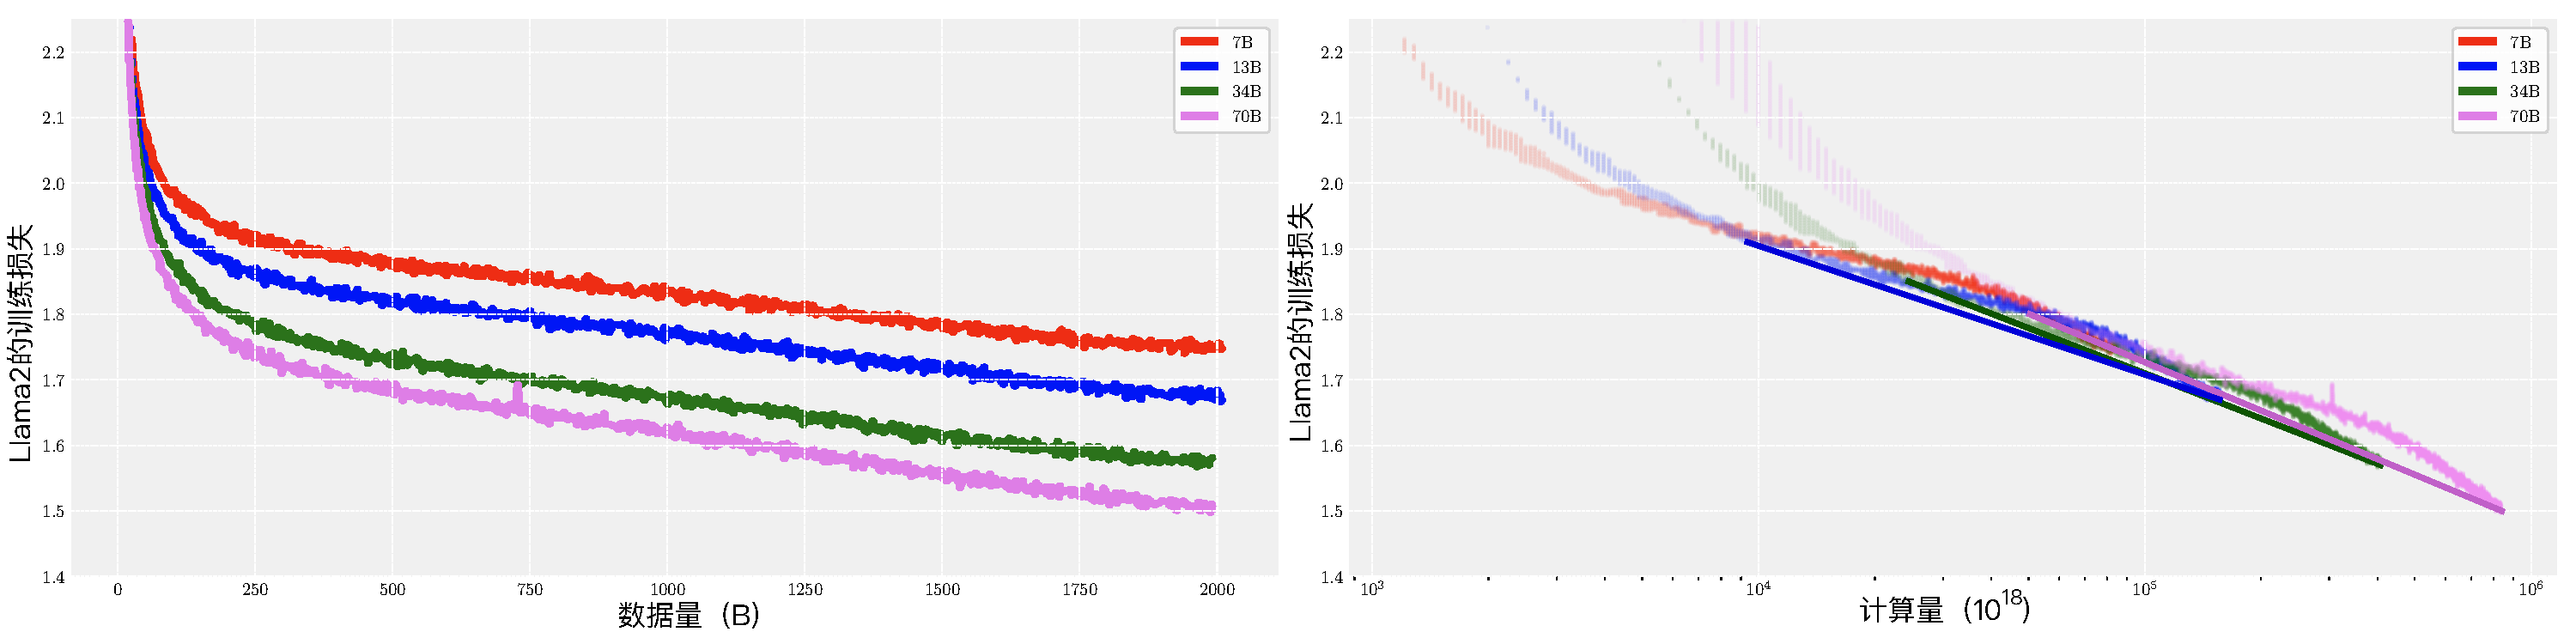
\includegraphics[width=1.0\textwidth]{minicpmFig/llama2_scaling.zh.pdf}
    \caption{根据Llama2的训练损失数据估计其计算最优比率}
    \label{fig:llamascaling}
\end{figure}




\subsection{分析}
\begin{figure}[htbp]
    \centering
    \begin{minipage}[b]{0.8\linewidth}
        \centering
        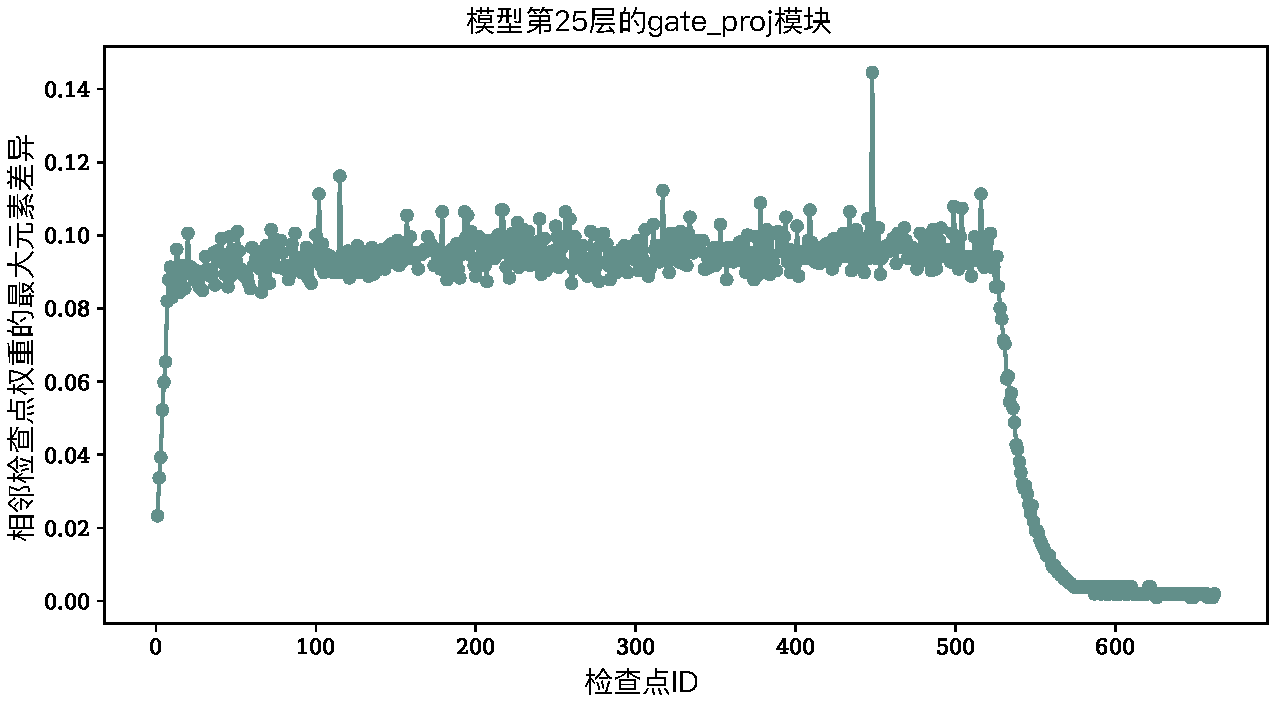
\includegraphics[width=1.0\linewidth]{minicpmFig/gate_proj_projection_vs_rank_25.zh.pdf}
    \end{minipage}
    \vspace{0.5cm} % 调整两个子图之间的间距
    \begin{minipage}[b]{0.8\linewidth}
        \centering
        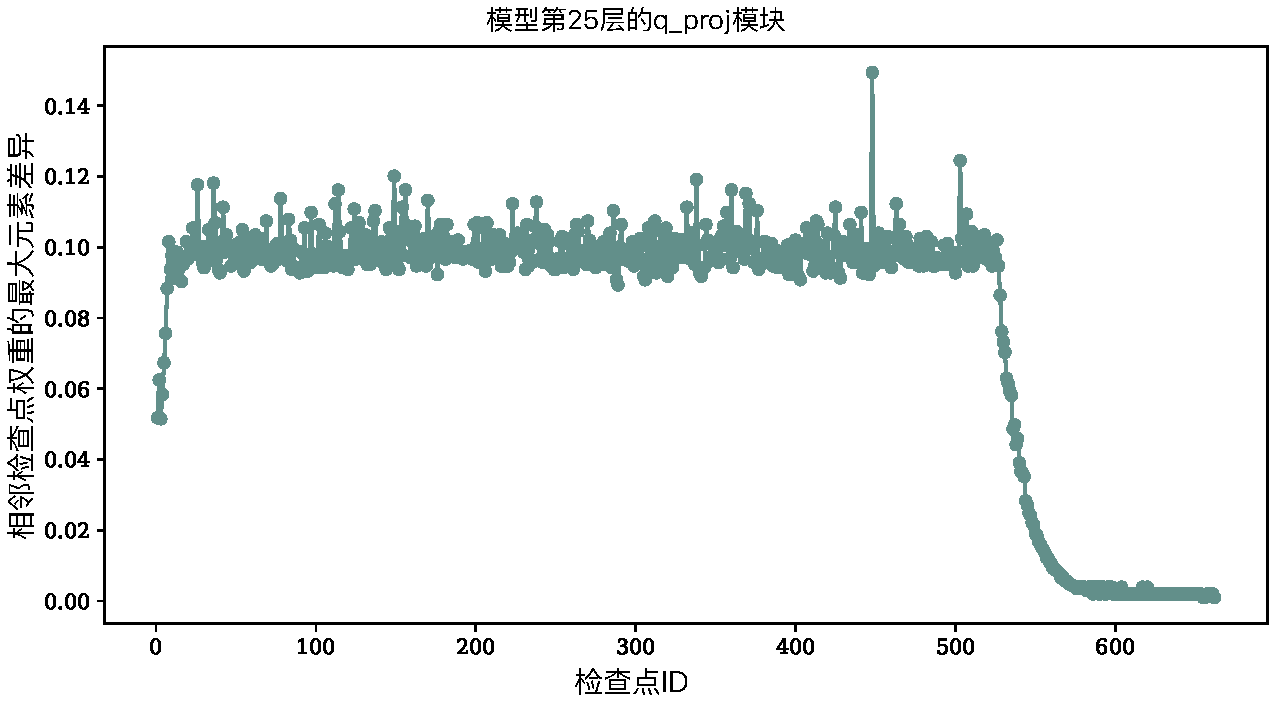
\includegraphics[width=1.0\linewidth]{minicpmFig/q_proj_projection_vs_rank_25.zh.pdf}
    \end{minipage}
    \caption{检查点的最大差异}
    \label{fig:appmaxdiff}
\end{figure}
本节从检查点更新和梯度信息的角度,对衰减阶段的损失下降进行简要分析。本文计算了MiniCPM - 2.4B(在\ref{sec:model}节中介绍)中所有权重矩阵的最大权重元素更新$max_{ij} (W_{ij}^{(t + 1)} - W_{ij}^{(t)})$。如图\ref{fig:appmaxdiff}所示,这些更新与学习率的大小呈现出很强的相关性。尽管图中展示的是两个子模块(第25层的gate\_proj和q\_proj模块),但这种模式在网络的每一层和子模块中都普遍存在。这一观察结果并非无足轻重:在学习率衰减之前,模型检查点经历了显著更新,但损失减少甚微。相反,在衰减阶段,尽管权重变化不太明显,但损失却加速下降。  




\begin{figure}[htbp]
    \centering
    % First minipage for the first figure
        \centering
        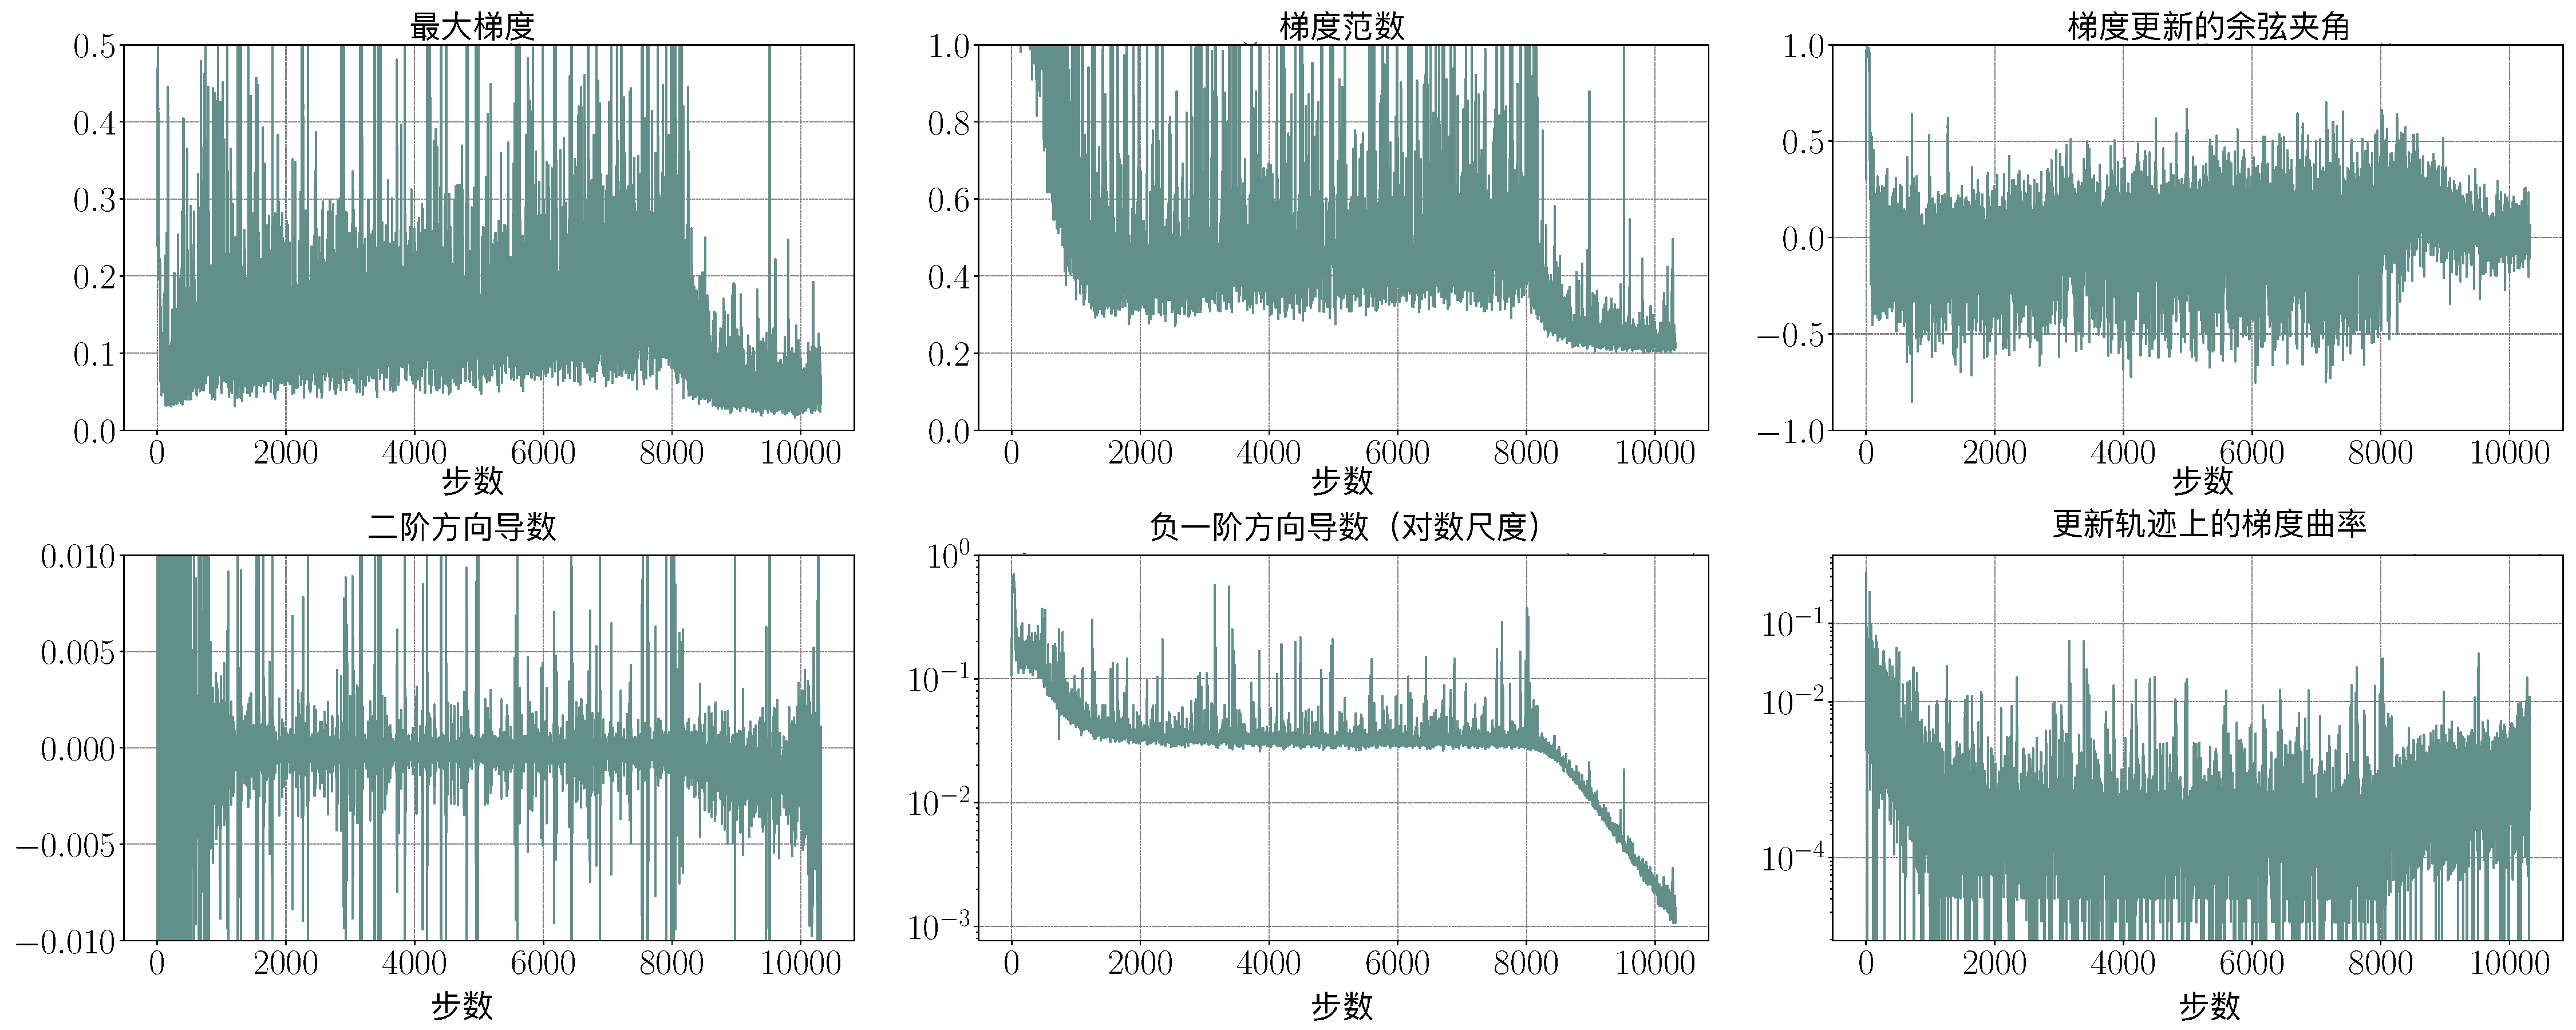
\includegraphics[width=1.0\linewidth]{minicpmFig/grad.pdf}
     \caption{0.2B模型使用WSD调度训练中的梯度相关统计量}
        \label{fig:grad}
\end{figure}

为了对梯度数据的进一步分析,本文训练了一个0.2B的模型,并详细记录了每一步的梯度信息,评估了连续步骤之间的差异,从而提供了二阶梯度信息的近似值。本文将第$t$步的梯度视为一个展平的向量$\mathbf{g}^{(t)}$,而第$t$步和第$t+1$步之间的参数(同样展平为向量$\mathbf{x}^{(t)}$)更新为$\mathbf{v}^{(t)} = \mathbf{x}^{(t+1)} - \mathbf{x}^{(t)}$。梯度范数取梯度的$L2$范数$\Vert\mathbf{g}^{(t)} \Vert$,梯度内积为$\mathbf{g}^{(t+1)} \cdot \mathbf{g}^{(t)}$,梯度角度的余弦由$\frac{\mathbf{g}^{(t+1)} \cdot \mathbf{g}^{(t)}}  {\Vert\mathbf{g}^{(t+1)} \Vert \Vert\mathbf{g}^{(t)} \Vert}$给出。将优化过程想象为在高维流形上的轨迹,沿轨迹的一阶方向导数为$D_1 = \frac{\mathbf{g}^{(t+1)} \cdot \mathbf{v}^{(t)}}{\|\mathbf{v}^{(t)}\|}
$,二阶方向导数为$D_2 = \frac{(\mathbf{g}^{(t+1)} - \mathbf{g}^{(t)}) \cdot \mathbf{v}^{(t)}}{\|\mathbf{v}^{(t)}\|^2}
$。$D_1, D_2$使得本文可以近似估计轨迹上的损失曲率,$K = \frac{|D_2|}{(1 + D_1^2)^{\frac{3}{2}}}$。这些统计量随时间的变化结果如图~\ref{fig:grad}所示,指数形式的退火阶段开始与8000步。可以看到,在衰减阶段,梯度范数逐渐减小,并且在此阶段开始时,梯度之间的余弦值主要为正,表明在衰减阶段,模型参数在步骤之间经历了一致的变化。关于方向导数,值得注意的是,一阶方向导数随着每一步呈指数级减小,与学习率高度一致,而二阶方向导数的幅度略有增加。损失函数的曲率也增加了一个数量级,表明接近局部最优解。这些发现可能为优化空间的形状提供了更深入的见解,这一主题留待未来探索。

